\documentclass[border=10pt]{standalone}
\usepackage{pgfplots}
\pgfplotsset{compat=1.18}
\begin{document}
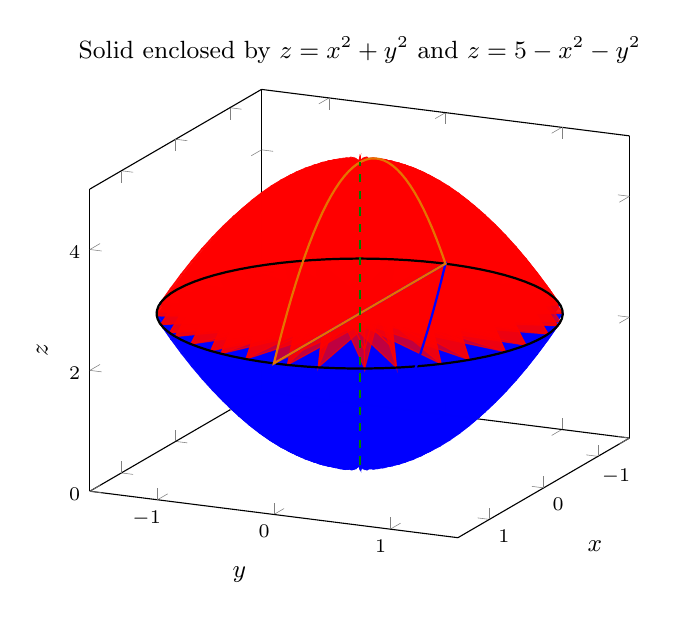
\begin{tikzpicture}
\begin{axis}[
    view={115}{20},
    xlabel={$x$}, ylabel={$y$}, zlabel={$z$},
    zmin=0, zmax=5,
    title={Solid enclosed by $z=x^2+y^2$ and $z=5-x^2-y^2$},
    tick label style={font=\scriptsize},
    label style={font=\small},
    title style={font=\small},
]
% Lower paraboloid z = r^2
\addplot3[surf, shader=flat, opacity=0.75, point meta=0,
    domain=0:1.5811, y domain=0:360, samples=20, samples y=40]
    ({x*cos(deg(y))}, {x*sin(deg(y))}, {x^2});
% Upper paraboloid z = 5 - r^2
\addplot3[surf, shader=flat, opacity=0.75, point meta=1,
    domain=0:1.5811, y domain=0:360, samples=20, samples y=40]
    ({x*cos(deg(y))}, {x*sin(deg(y))}, {5-x^2});
% Intersection circle at z = 2.5
\addplot3[black, thick, domain=0:360, samples=80, variable=\t]
    ({1.5811*cos(\t)}, {1.5811*sin(\t)}, {2.5});
% Slice curves at y=0
\addplot3[blue, thick, domain=-1.5811:1.5811, samples=40] ({x}, {0}, {x^2});
\addplot3[orange!90!black, thick, domain=-1.5811:1.5811, samples=40] ({x}, {0}, {5-x^2});
% z-axis
\addplot3[green!50!black, dashed, thick] coordinates {(0,0,0) (0,0,5)};
\end{axis}
\end{tikzpicture}
\end{document}
